\begin{lstlisting}
p110 8 (6)(7)(8)(10)(12)(13)(14)
p111 11 12 14 15
\end{lstlisting}
\begin{exercise}
\begin{figure}[H]
\centering
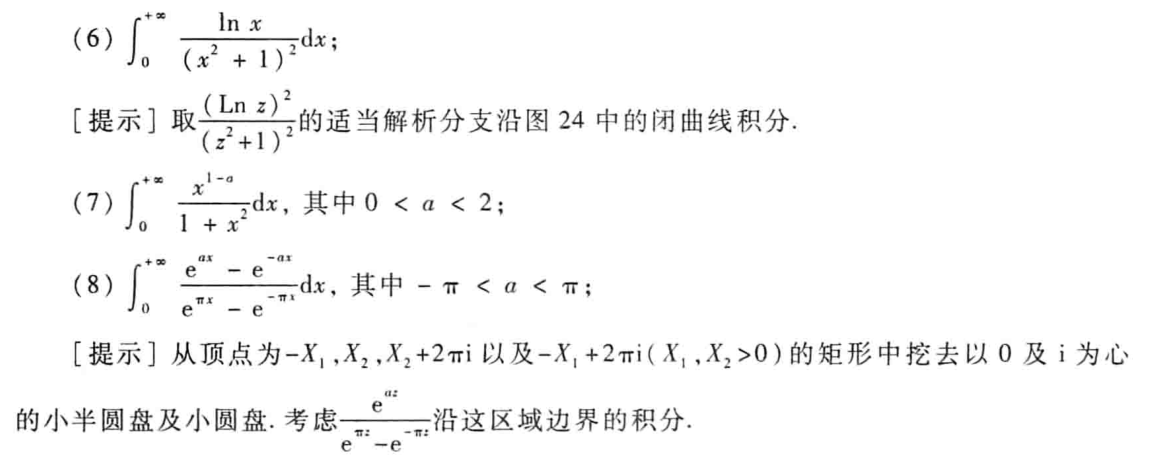
\includegraphics[width=\textwidth]{1-hw11-2025051222.png}
% \caption{}
\label{}
\end{figure}
\end{exercise}
(6) $-\frac{\pi}{4}$

(7) $\frac{1}{2}\pi \csc\left( \frac{a\pi}{2} \right)$

(8) $\frac{1}{2}\tan\left( \frac{a}{2} \right)$

\begin{exercise}
\begin{figure}[H]
\centering
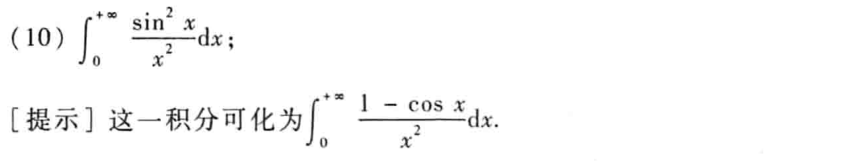
\includegraphics[width=\textwidth]{3-hw11-2025051222.png}
% \caption{}
\label{}
\end{figure}
\end{exercise}
\begin{figure}[H]
\centering
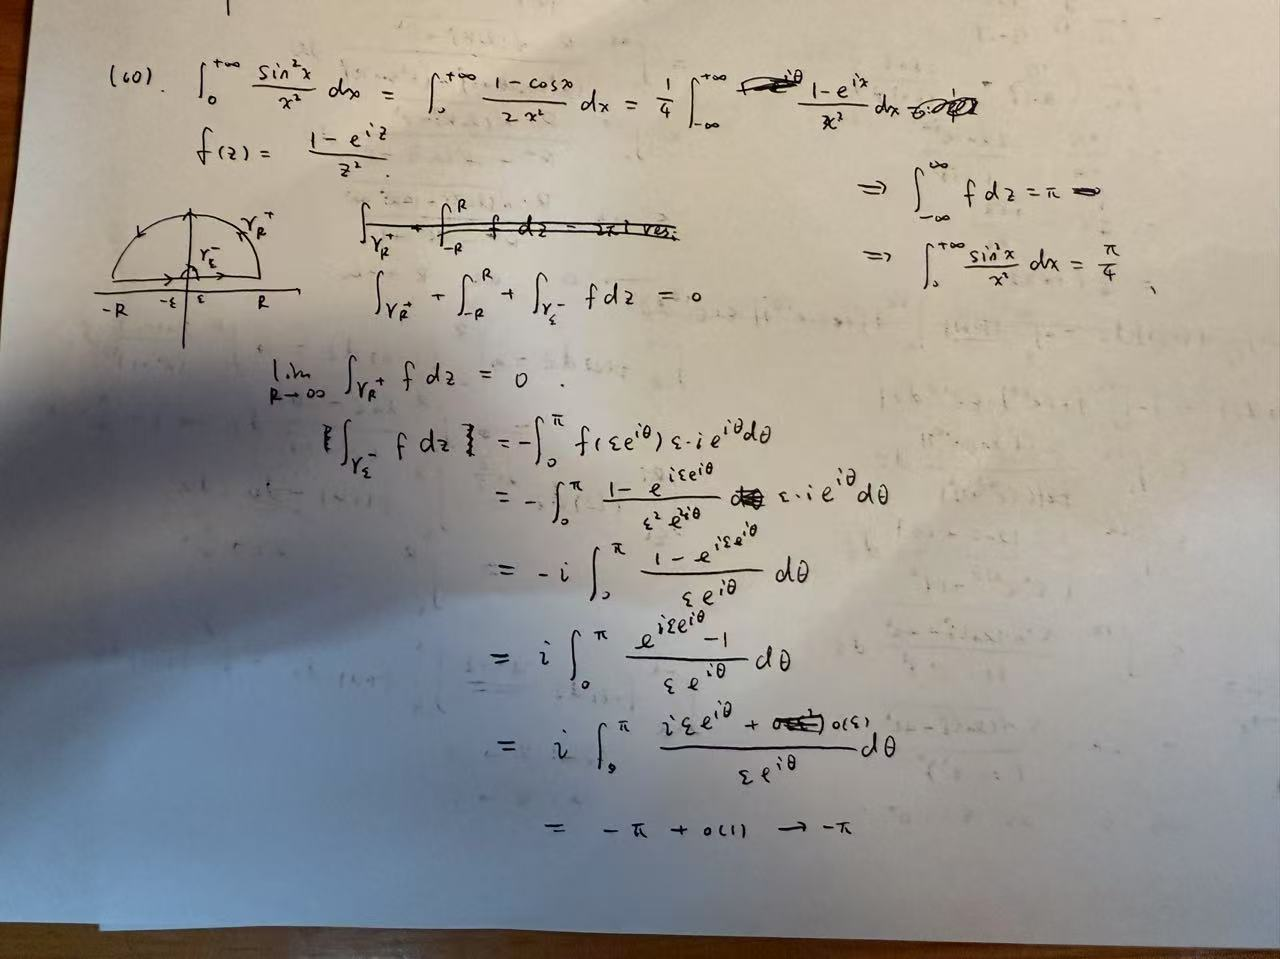
\includegraphics[width=\textwidth]{e4aa87a842ea72501199a17e1558455c.jpg}
% \caption{}
\label{}
\end{figure}

\begin{exercise}
\begin{figure}[H]
\centering
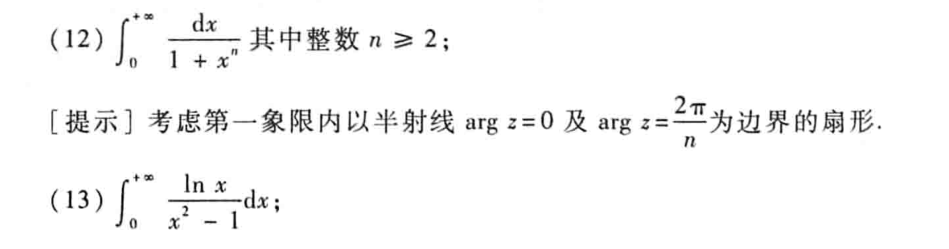
\includegraphics[width=\textwidth]{2-hw11-2025051222.png}
% \caption{}
\label{}
\end{figure}
\end{exercise}
(12) $\frac{\pi}{n}\csc \frac{\pi}{n}$.

(13) $\frac{\pi^{2}}{4}$.

\begin{figure}[H]
\centering
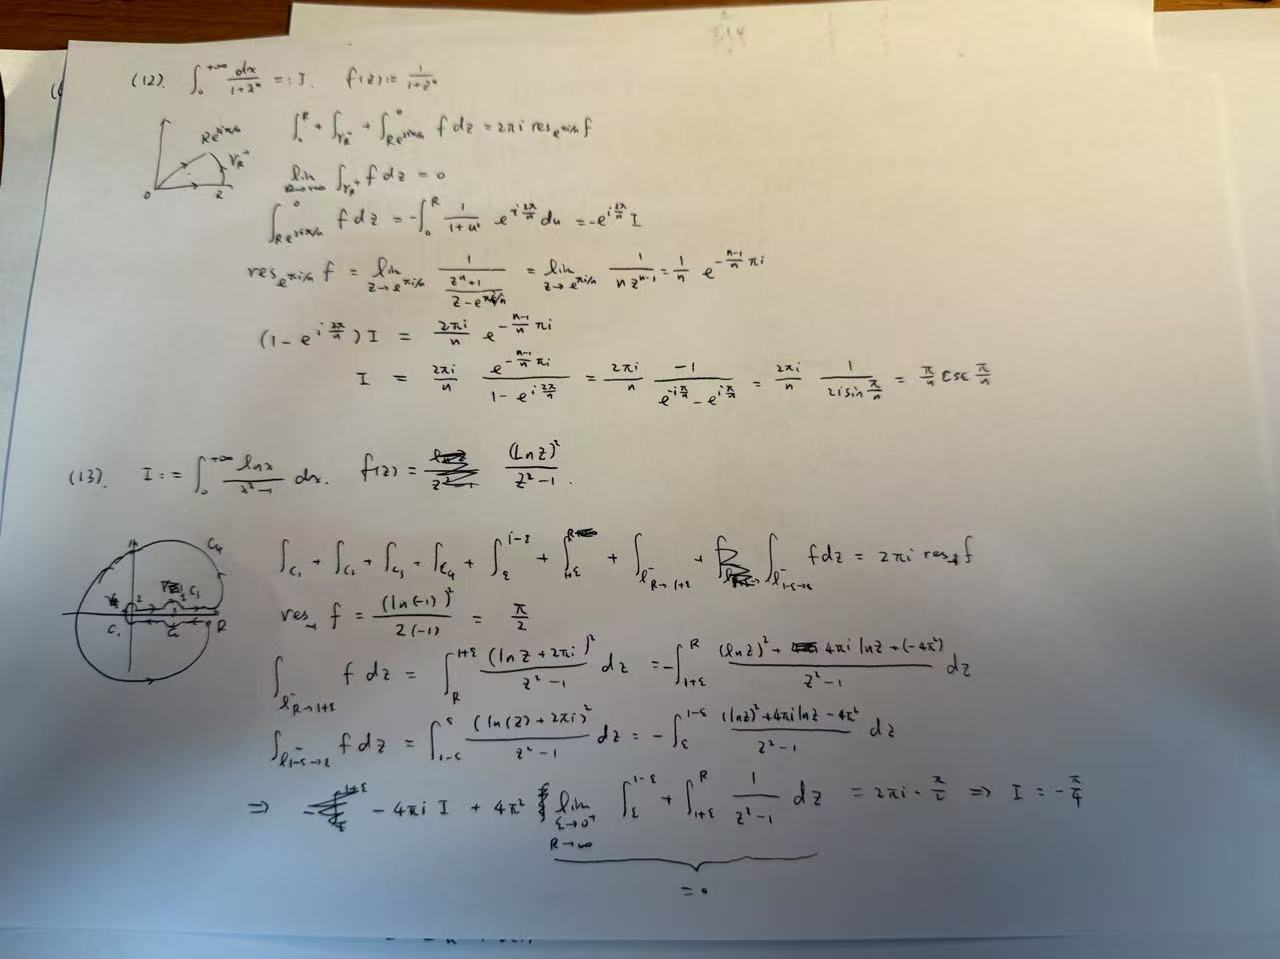
\includegraphics[width=\textwidth]{3ae846ce63aa5cfd332852fc20c2e6f7.jpg}
% \caption{}
\label{}
\end{figure}

\begin{exercise}
\begin{figure}[H]
\centering
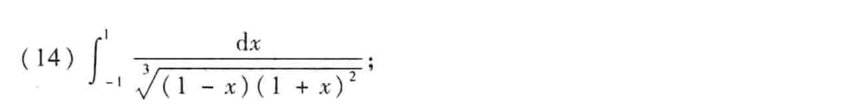
\includegraphics[width=\textwidth]{4-hw11-2025051222.png}
% \caption{}
\label{}
\end{figure}
\end{exercise}
\[
\frac{8\pi}{9\sqrt{ 3 }}
\]
\begin{exercise}
\begin{figure}[H]
\centering
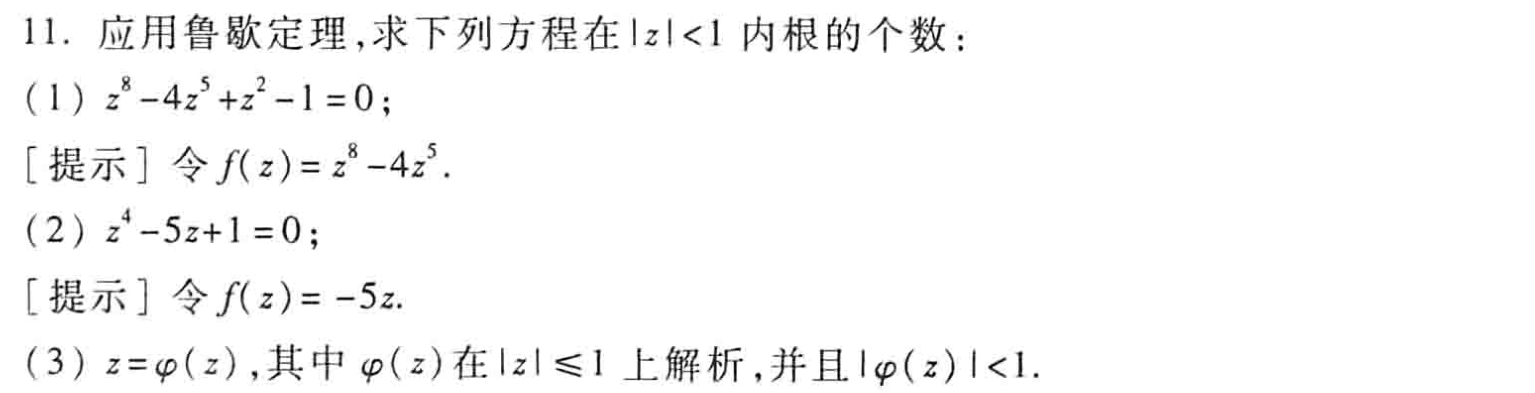
\includegraphics[width=\textwidth]{5-hw11-2025051222.png}
% \caption{}
\label{}
\end{figure}
\end{exercise}
\begin{figure}[H]
\centering
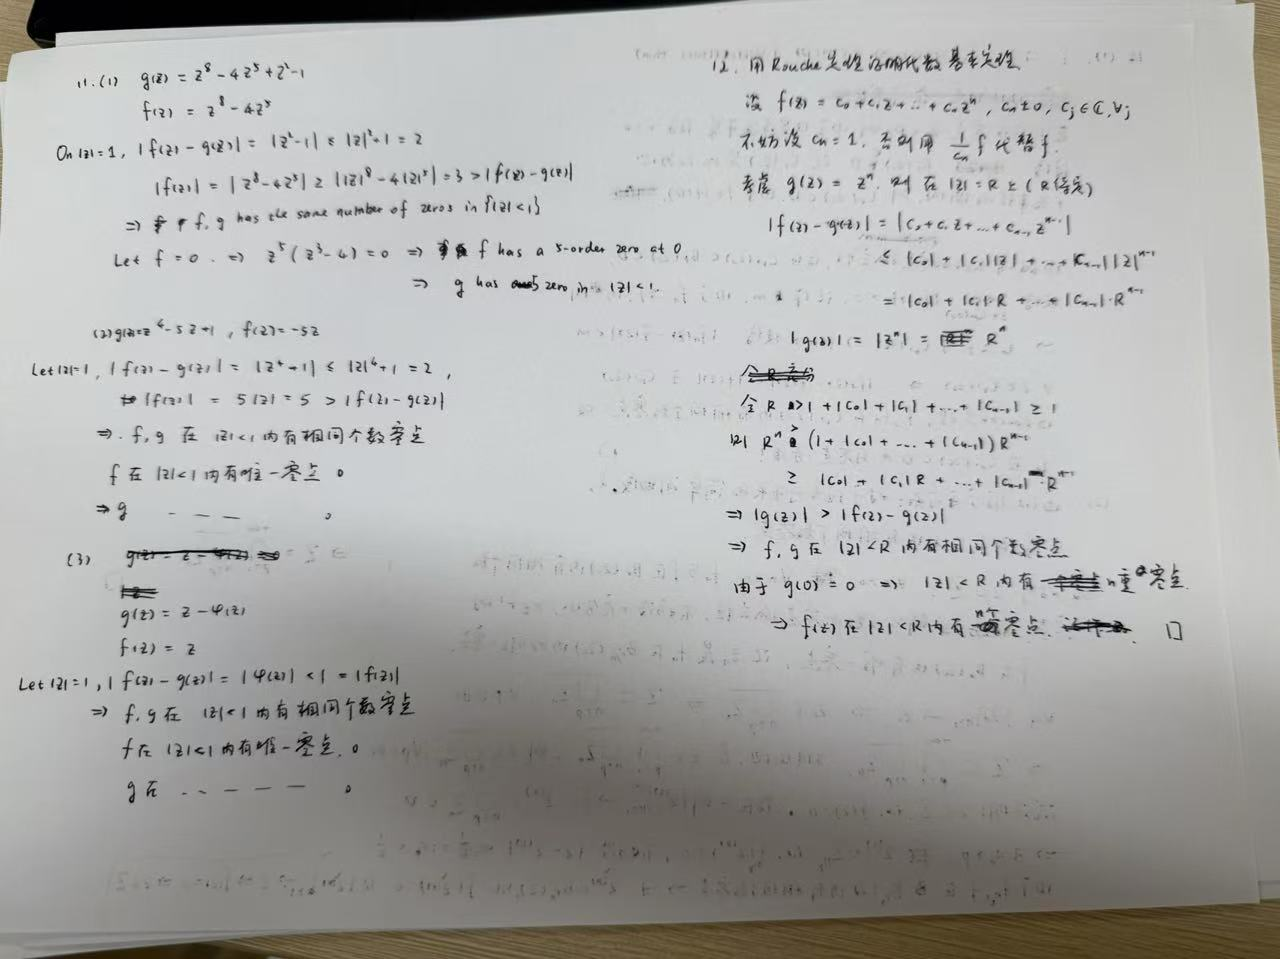
\includegraphics[width=\textwidth]{99f6b691971bbe6f3052a1503163e3d3.jpg}
% \caption{}
\label{}
\end{figure}

\begin{exercise}
\begin{figure}[H]
\centering
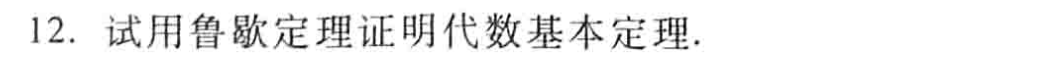
\includegraphics[width=\textwidth]{6-hw11-2025051222.png}
% \caption{}
\label{}
\end{figure}
\end{exercise}
\begin{figure}[H]
\centering
\includegraphics[width=\textwidth]{99f6b691971bbe6f3052a1503163e3d3 1.jpg}
% \caption{}
\label{}
\end{figure}

\begin{exercise}
\begin{figure}[H]
\centering
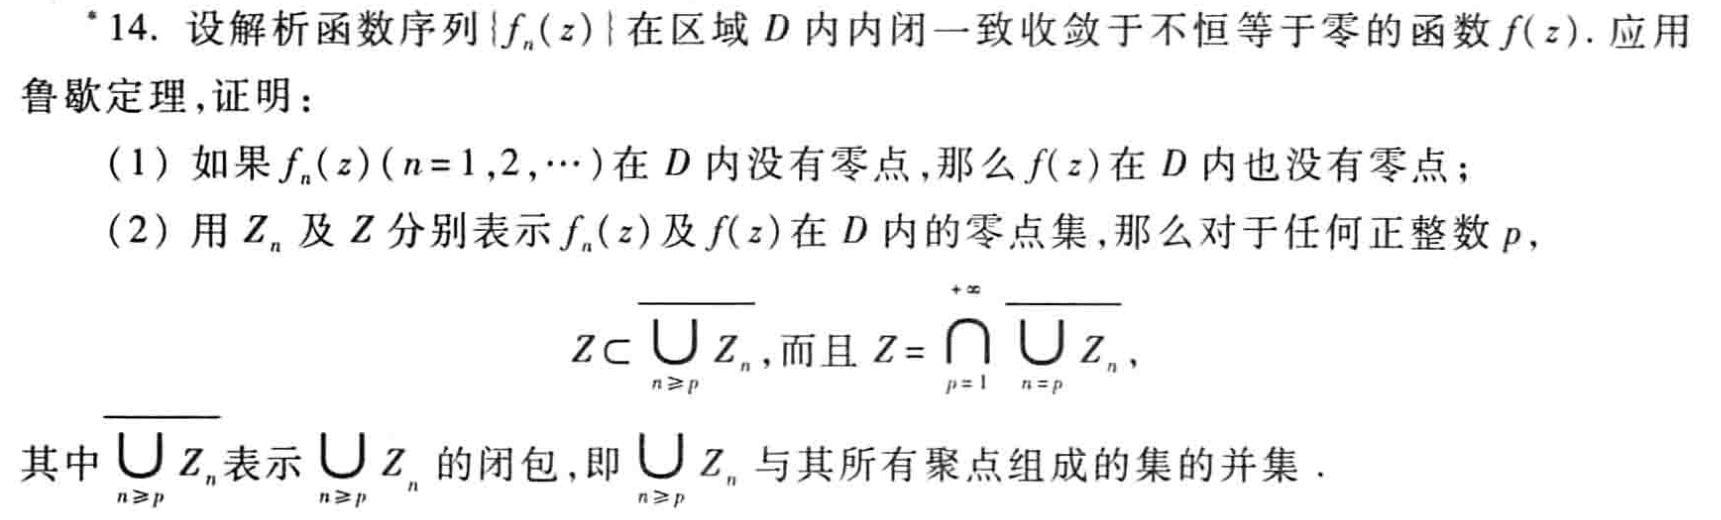
\includegraphics[width=\textwidth]{7-hw11-2025051222.png}
% \caption{}
\label{}
\end{figure}
\end{exercise}
\begin{figure}[H]
\centering
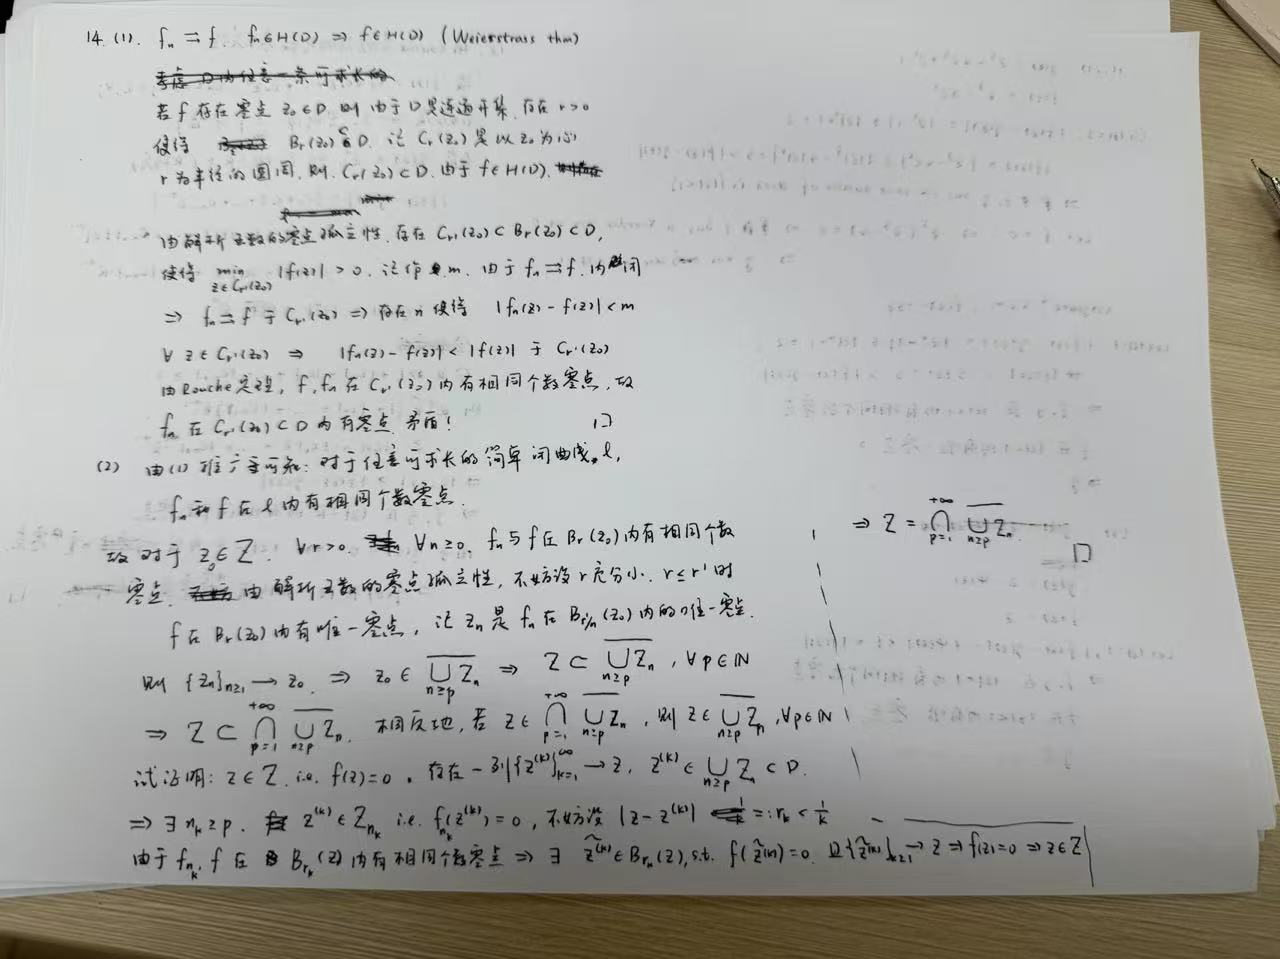
\includegraphics[width=\textwidth]{3019c9996e90f823fa10aaca79a20fd0.jpg}
% \caption{}
\label{}
\end{figure}

\begin{exercise}
\begin{figure}[H]
\centering
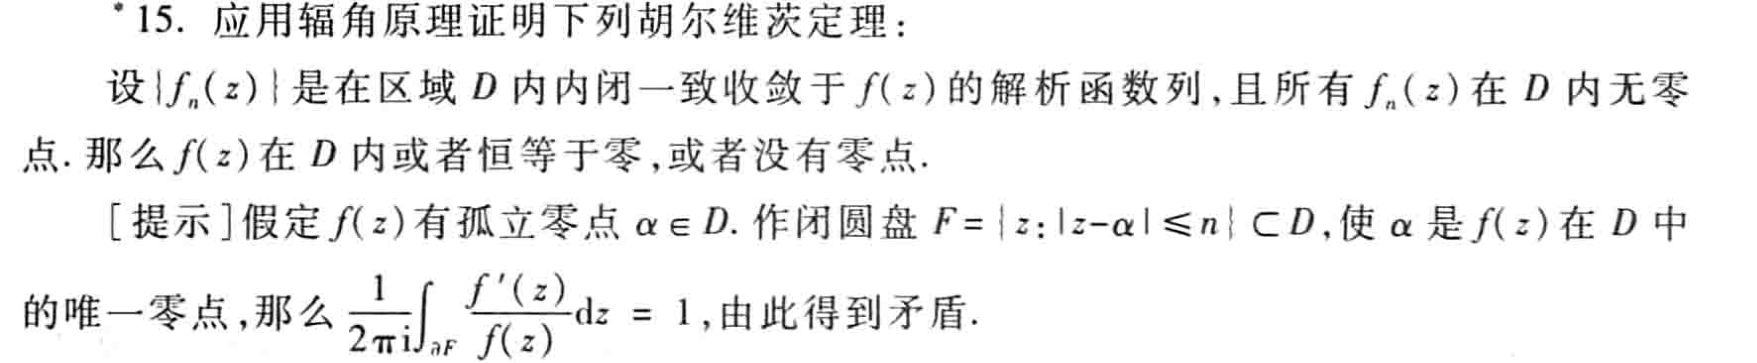
\includegraphics[width=\textwidth]{8-hw11-2025051222.png}
% \caption{}
\label{}
\end{figure}
\end{exercise}
假设有一个复变函数 $f(z)$,它在一条简单闭合曲线 $C$ 的内部及边界上是解析的(除了有限个极点外),并且在 $C$ 上没有零点和极点。那么,当 $z$ 沿着曲线 $C$ 逆时针方向绕行一周时,$f(z)$ 的辐角变化量等于 $2\pi$ 乘以函数 $f(z)$ 在曲线 $C$ 内部零点的个数(计重数)减去极点的个数(计重数)。
用公式表示:
\[
\Delta_C \arg f(z) = 2\pi(N - P)
\]
其中:

\begin{itemize}
	\item $\Delta_C \arg f(z)$ 表示当 $z$ 沿曲线 $C$ 逆时针方向绕行一周时,$f(z)$ 的辐角变化量。
	\item $N$ 表示函数 $f(z)$ 在曲线 $C$ 内部零点的个数(如果一个零点是 $k$ 重的,则计为 $k$ 个)。
	\item $P$ 表示函数 $f(z)$ 在曲线 $C$ 内部极点的个数(如果一个极点是 $k$ 重的,则计为 $k$ 个)。
\end{itemize}

另一种等价的表述形式是利用对数导数:
\[
\frac{1}{2\pi i} \oint_C \frac{f'(z)}{f(z)} \, dz = N - P
\]
这个积分实际上计算了 $f(z)$ 的像在原点周围缠绕的圈数。

\begin{figure}[H]
\centering
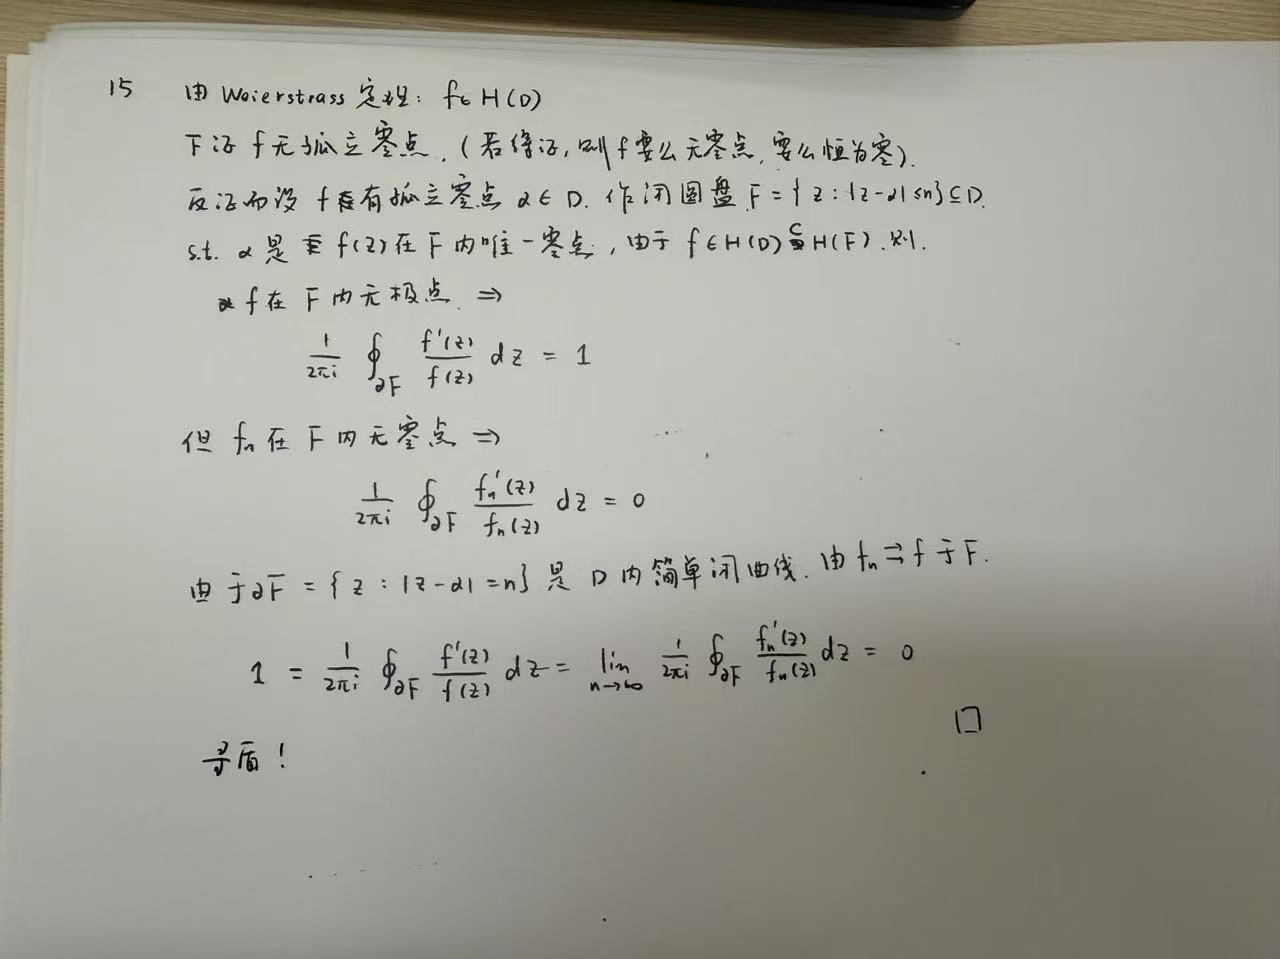
\includegraphics[width=\textwidth]{15e68e8704605b6d0579751f181ee127.jpg}
% \caption{}
\label{}
\end{figure}
